\documentclass{article}
\usepackage{amsmath}
\usepackage{amssymb}
\usepackage{graphicx}
\usepackage{tikz}
\usepackage{pgfplots}
\usepackage{float}
\usepackage{subcaption}
\usepackage{geometry}

\geometry{a4paper, margin=1in}

% Define example environment
\newenvironment{example}[1]{
    \begin{trivlist}
    \item[\textbf{Example:}] #1
    \vspace{0.5em}
}{
    \end{trivlist}
    \vspace{1em}
}

\pgfplotsset{compat=1.18}
\usetikzlibrary{patterns,decorations.pathreplacing}

\title{Lecture 2 Examples}
\author{Signals and Systems Course}
\date{}

\begin{document}

\maketitle

\begin{example}[1. Fundamental Periodicity of a Continuous-Time Sinusoid]
\textbf{Problem:}
Show that $x(t) = A \cos(\omega_0 t + \theta)$ is periodic with fundamental period $T_0 = 2\pi/\omega_0$.

\begin{figure}[H]
    \centering
    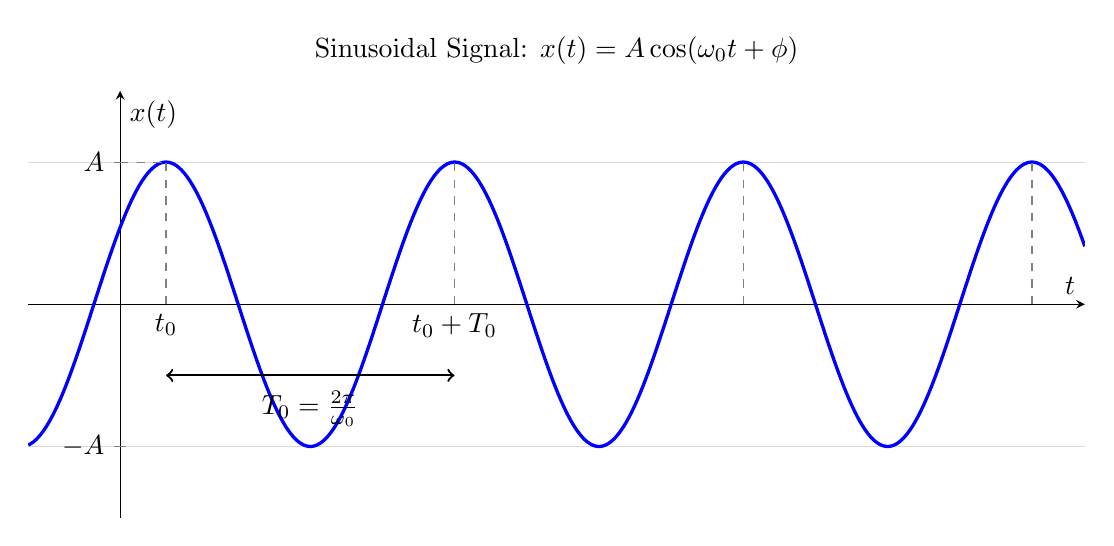
\begin{tikzpicture}
	\begin{axis}[
		% Set the overall style (wider to accommodate more cycles)
		width=15cm,
		height=7cm,
		% Title with the general function
		title={Sinusoidal Signal: $x(t) = A \cos(\omega_0 t + \phi)$},
		% Axis labels
		xlabel={$t$},
		ylabel={$x(t)$},
		% Position axes at the origin
		axis lines=middle,
		% Set axis limits to show three cycles
		xmin=-2, xmax=21,
		ymin=-1.5, ymax=1.5,
		% Disable default ticks to add custom symbolic ones
		xtick=\empty,
		ytick=\empty,
		extra y ticks={-1, 1},
		extra y tick labels={$-A$, $A$},
		% Add a grid
		grid=major,
		grid style={line width=.1pt, draw=gray!30},
		% Plotting settings
		domain=-2:21,
		samples=400, % Increased samples for a smooth curve over the larger domain
		no marks,
		]
		
		% Plot a representative cosine wave (A=1, w0=1, phi=-1 rad)
		\addplot[blue, very thick] {cos(deg(x - 1))};
		
		% --- ANNOTATIONS ---
		
		% 1. Mark the Period (T_0) between the first two peaks
		% First peak is at t=1. Period is 2*pi. Second peak is at t = 1 + 2*pi ~ 7.28
		\draw[dashed, gray] (axis cs:1,0) -- (axis cs:1,1);
		\draw[dashed, gray] (axis cs:7.28,0) -- (axis cs:7.28,1);
		
		% Add a double-arrow line to label the period
		\draw[<->, thick] (axis cs:1, -0.5) -- (axis cs:7.28, -0.5) node[midway, below=2pt] {$T_0 = \frac{2\pi}{\omega_0}$};
		
		% 2. Mark the Amplitude (A)
		% Add a guideline from the first peak to the y-axis
		\draw[dashed, gray] (axis cs:0,1) -- (axis cs:1,1);
		
		% 3. Label key time instances for the first two peaks
		\node[below] at (axis cs:1, 0) {$t_0$};
		\node[below] at (axis cs:7.28, 0) {$t_0+T_0$};
		
		% 4. Add guidelines for the subsequent peaks to show the full three cycles
		% Third peak: t = 1 + 4*pi ~ 13.57
		% Fourth peak: t = 1 + 6*pi ~ 19.85
		\draw[dashed, gray] (axis cs:13.57,0) -- (axis cs:13.57,1);
		\draw[dashed, gray] (axis cs:19.85,0) -- (axis cs:19.85,1);
		
	\end{axis}
\end{tikzpicture}
    \caption{A generic plot of the continuous-time sinusoidal signal $x(t) = A \cos(\omega_0 t + \theta)$, illustrating its periodicity.}
\end{figure}

\textbf{Solution:}

For periodicity: $x(t + T_0) = x(t)$

$$x(t + T_0) = A \cos(\omega_0 (t + T_0) + \theta) = A \cos(\omega_0 t + \omega_0 T_0 + \theta)$$

For $x(t + T_0) = x(t)$: $\omega_0 T_0 = 2\pi k$ for integer $k$

The smallest positive $T_0$ occurs when $k = 1$:

$$T_0 = \frac{2\pi}{\omega_0}$$

\textbf{Answer:} $T_0 = \frac{2\pi}{\omega_0}$
\end{example}

\vspace{0.5em}
\hrule
\vspace{0.5em}

\begin{example}[2. Periodicity of the Sum of Continuous-Time Signals]
\textbf{Problem:}
Given:
\begin{align}
    x_1(t) &= \sin(10\pi t) \\
    x_2(t) &= \sin(20\pi t) \\
    x_3(t) &= \sin(31t)
\end{align}

Determine if $x_4(t) = x_1(t) + x_2(t)$ and $x_5(t) = x_1(t) + x_3(t)$ are periodic. If periodic, find the fundamental period.

\textbf{Solution:}

\textbf{Fundamental periods:}
\begin{align}
T_1 &= \frac{2\pi}{10\pi} = \frac{1}{5} \\
T_2 &= \frac{2\pi}{20\pi} = \frac{1}{10} \\
T_3 &= \frac{2\pi}{31}
\end{align}

\textbf{For $x_4(t) = x_1(t) + x_2(t)$:}
$$\frac{T_1}{T_2} = \frac{1/5}{1/10} = 2$$

Since the ratio is rational, $x_4(t)$ is periodic with $T_4 = \frac{1}{5}$.

\textbf{For $x_5(t) = x_1(t) + x_3(t)$:}
$$\frac{T_1}{T_3} = \frac{1/5}{2\pi/31} = \frac{31}{10\pi}$$

Since the ratio is irrational, $x_5(t)$ is not periodic.

\begin{figure}[H]
    \centering
    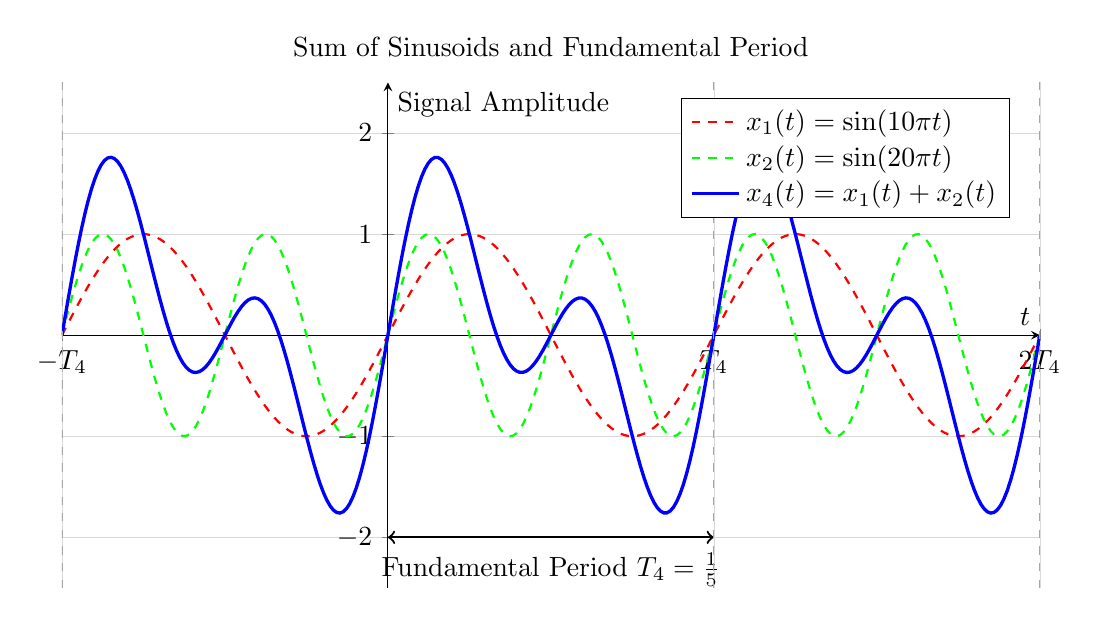
\begin{tikzpicture}
	\begin{axis}[
		% Set the overall style
		width=14cm,
		height=8cm,
		title={Sum of Sinusoids and Fundamental Period},
		% Axis labels
		axis lines=middle,
		xlabel={$t$},
		ylabel={Signal Amplitude},
		% Set axis limits to show one negative and two positive cycles
		xmin=-0.2, xmax=0.4,
		ymin=-2.5, ymax=2.5,
		% Use symbolic ticks including the negative period
		xtick={-0.2, 0.2, 0.4},
		xticklabels={$-T_4$, $T_4$, $2T_4$},
		ytick={-2, -1, 1, 2},
		% Add a grid
		grid=major,
		grid style={line width=.1pt, draw=gray!30},
		% Plotting settings
		domain=-0.2:0.4,
		samples=300,
		no marks,
		% Legend settings
		legend pos=north east,
		legend cell align={left},
		]
		
		% Plot the two component sinusoids (dashed and less thick)
		\addplot[red, thick, dashed] {sin(deg(10*pi*x))};
		\addlegendentry{$x_1(t) = \sin(10\pi t)$};
		
		\addplot[green, thick, dashed] {sin(deg(20*pi*x))};
		\addlegendentry{$x_2(t) = \sin(20\pi t)$};
		
		% Plot the sum (solid and very thick to emphasize it)
		\addplot[blue, very thick] {sin(deg(10*pi*x)) + sin(deg(20*pi*x))};
		\addlegendentry{$x_4(t) = x_1(t) + x_2(t)$};
		
		% Add a double-arrow line below the axis to mark the fundamental period
		\draw[<->, thick] (axis cs:0, -2) -- (axis cs:0.2, -2) 
		node[midway, below=2pt] {Fundamental Period $T_4 = \frac{1}{5}$};
		
		% Add subtle vertical lines to guide the eye at each period
		\draw[dashed, gray!70] (axis cs:-0.2, -2.5) -- (axis cs:-0.2, 2.5);
		\draw[dashed, gray!70] (axis cs:0.2, -2.5) -- (axis cs:0.2, 2.5);
		\draw[dashed, gray!70] (axis cs:0.4, -2.5) -- (axis cs:0.4, 2.5);
		
	\end{axis}
\end{tikzpicture}
    \caption{A plot of $x_4(t)$. We can see that $x_1(t)$ (with period $T_1=1/5$) completes one cycle while $x_2(t)$ (with period $T_2=1/10$) completes two cycles. The sum signal $x_4(t)$ repeats every $T_4=1/5$ seconds.}
    \label{fig:x4}
\end{figure}

\textbf{Answer:} $x_4(t)$ is periodic with $T_4 = \frac{1}{5}$; $x_5(t)$ is not periodic.
\end{example}

\vspace{0.5em}
\hrule
\vspace{0.5em}

\begin{example}[3. Even and Odd Decomposition of a Triangular Pulse]
\textbf{Problem:}
Given the continuous-time signal $x(t)$ shown below, find its even component, $x_e(t)$, and its odd component, $x_o(t)$.

The signal $x(t)$ is a triangular pulse defined mathematically as:
\[
x(t) = \begin{cases}
    t & \text{for } 0 \le t \le 1 \\
    2-t & \text{for } 1 < t \le 2 \\
    0 & \text{otherwise}
\end{cases}
\]

\begin{figure}[H]
    \centering
    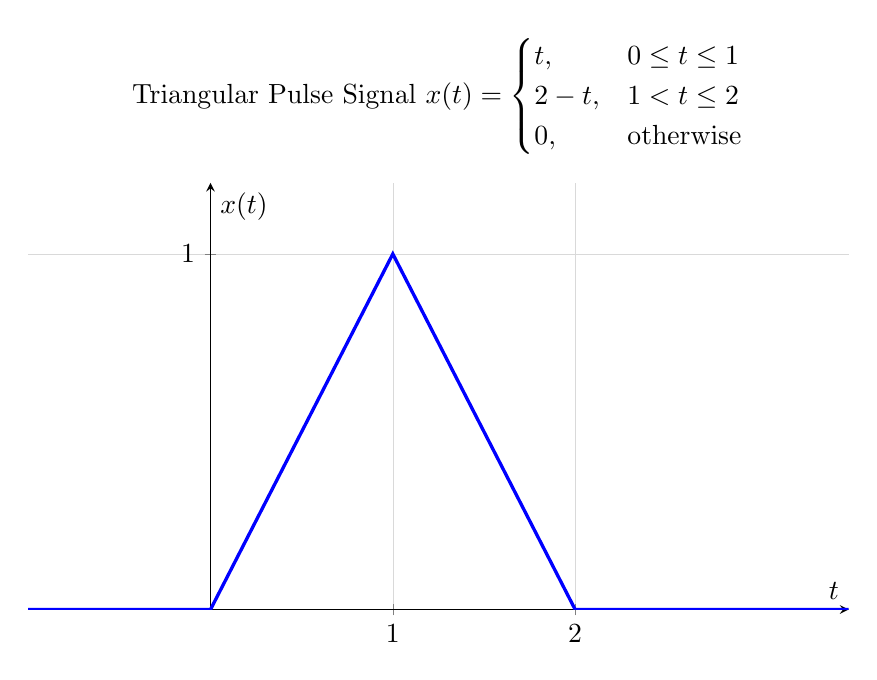
\begin{tikzpicture}
	\begin{axis}[
		% Set the overall style
		width=12cm,
		height=7cm,
		% Title with the formal piecewise definition
		title={Triangular Pulse Signal $x(t) = 
			\begin{cases} 
				t, & 0 \le t \le 1 \\
				2-t, & 1 < t \le 2 \\
				0, & \text{otherwise} 
			\end{cases}$
		},
		% Axis labels
		xlabel={$t$},
		ylabel={$x(t)$},
		% Position axes at the origin
		axis lines=middle,
		% Set axis limits for good spacing
		xmin=-1, xmax=3.5,
		ymin=0, ymax=1.2,
		% Set ticks at key points
		xtick={1, 2},
		ytick={1},
		yticklabels={$1$},
		% Add a grid
		grid=major,
		grid style={line width=.1pt, draw=gray!30},
		]
		
		% Draw the entire signal shape using a single command
		\draw[blue, very thick]
		(axis cs:-1, 0) -- (axis cs:0, 0)   % Zero before t=0
		-- (axis cs:1, 1)                   % Ramp up to the peak at t=1
		-- (axis cs:2, 0)                   % Ramp down to zero at t=2
		-- (axis cs:3.5, 0);                 % Zero after t=2
		
	\end{axis}
\end{tikzpicture}
    \caption{The original triangular pulse signal $x(t)$.}
    \label{fig:xt}
\end{figure}

\textbf{Solution:}

Any signal can be decomposed into even and odd components:
\[ x_e(t) = \frac{1}{2} [x(t) + x(-t)], \quad x_o(t) = \frac{1}{2} [x(t) - x(-t)] \]

\textbf{Step 1: Find $x(-t)$}
Reflect $x(t)$ about $t=0$: $x(-t)$ exists for $t \in [-2, 0]$.

\begin{figure}[H]
    \centering
    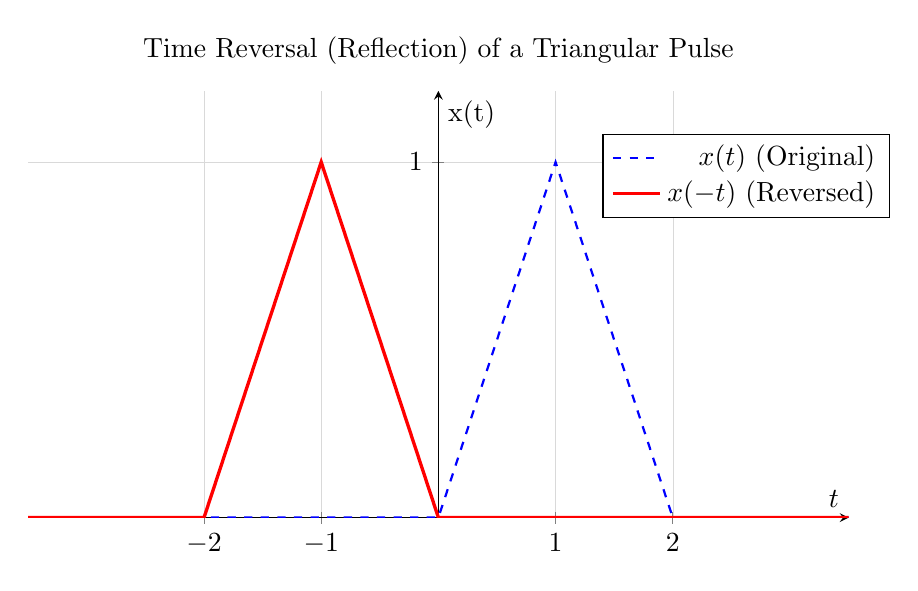
\begin{tikzpicture}
	\begin{axis}[
		% Set the overall style
		width=12cm,
		height=7cm,
		% Title describing the transformation
		title={Time Reversal (Reflection) of a Triangular Pulse},
		% Axis labels
		xlabel={$t$},
		ylabel={x(t)},
		% Position axes at the origin
		axis lines=middle,
		% Set axis limits to show both signals
		xmin=-3.5, xmax=3.5,
		ymin=0, ymax=1.2,
		% Set ticks at key points for both signals
		xtick={-2, -1, 1, 2},
		ytick={1},
		yticklabels={$1$},
		% Add a grid
		grid=major,
		grid style={line width=.1pt, draw=gray!30},
		% Position the legend
		legend style={
			at={(0.7, 0.9)}, % 3% from left, 97% from bottom
			anchor=north west,   % Anchor the top-left corner of the legend
			legend cell align={right}
		},
		]
		
		% 1. Plot the original signal (dashed blue) for reference
		\addplot[blue, dashed, thick] coordinates {
			(-3.5,0) (0,0) (1,1) (2,0) (3.5,0)
		};
		\addlegendentry{$x(t)$ (Original)};
		
		% 2. Plot the time-reversed signal (solid red)
		\addplot[red, very thick] coordinates {
			(-3.5,0) (-2,0) (-1,1) (0,0) (3.5,0)
		};
		\addlegendentry{$x(-t)$ (Reversed)};
		
	\end{axis}
\end{tikzpicture}
    \caption{The time-reversed signal $x(-t)$, obtained by reflecting $x(t)$ about the vertical axis.}
    \label{fig:x_neg_t}
\end{figure}

\textbf{Step 2: Calculate $x_e(t)$}
For $t > 0$: $x_e(t) = \frac{1}{2} x(t)$ (since $x(-t)=0$)
For $t < 0$: $x_e(t) = \frac{1}{2} x(-t)$ (since $x(t)=0$)
At $t=0$: $x_e(0) = 0$

\begin{figure}[H]
    \centering
    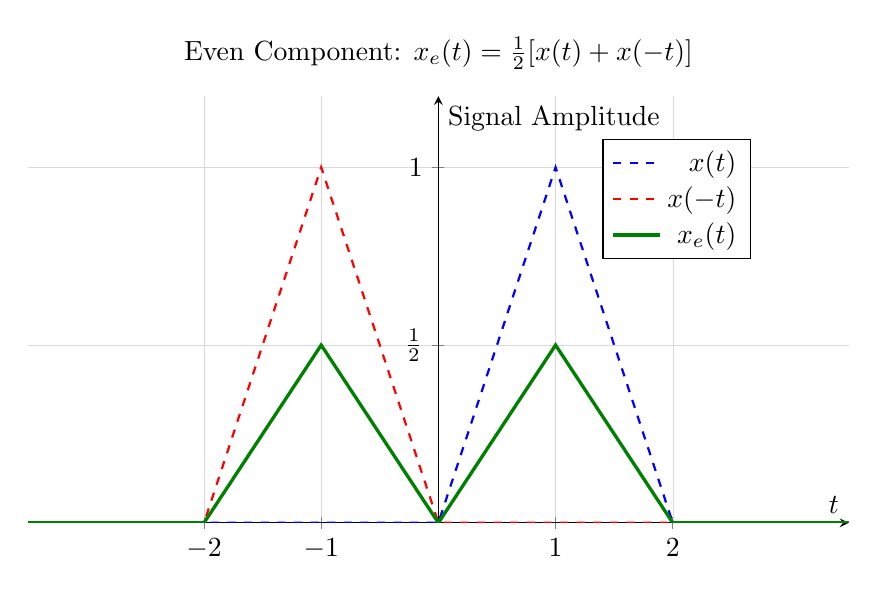
\begin{tikzpicture}
	\begin{axis}[
		% Set the overall style
		width=12cm,
		height=7cm,
		% Title with the definition of the even component
		title={Even Component: $x_e(t) = \frac{1}{2}[x(t) + x(-t)]$},
		% Axis labels
		xlabel={$t$},
		ylabel={Signal Amplitude},
		% Position axes at the origin
		axis lines=middle,
		% Set axis limits to show all signals
		xmin=-3.5, xmax=3.5,
		ymin=0, ymax=1.2,
		% Set ticks at key points
		xtick={-2, -1, 1, 2},
		ytick={0.5, 1},
		yticklabels={$\frac{1}{2}$, $1$},
		% Add a grid
		grid=major,
		grid style={line width=.1pt, draw=gray!30},
		% Position the legend
		legend style={
		at={(0.7, 0.9)}, % 3% from left, 97% from bottom
		anchor=north west,   % Anchor the top-left corner of the legend
		legend cell align={right}
	},
		]
		
		% 1. Plot the original signal (dashed blue)
		\addplot[blue, dashed, thick] coordinates {
			(-3.5,0) (0,0) (1,1) (2,0) (3.5,0)
		};
		\addlegendentry{$x(t)$};
		
		% 2. Plot the time-reversed signal (dashed red)
		\addplot[red, dashed, thick] coordinates {
			(-3.5,0) (-2,0) (-1,1) (0,0) (3.5,0)
		};
		\addlegendentry{$x(-t)$};
		
		% 3. Plot the resulting even component (solid green)
		\addplot[green!50!black, very thick] coordinates {
			(-3.5,0) (-2,0) (-1,0.5) (0,0) (1,0.5) (2,0) (3.5,0)
		};
		\addlegendentry{$x_e(t) $};
		
	\end{axis}
\end{tikzpicture}
    \caption{The even component $x_e(t) = \frac{1}{2}[x(t)+x(-t)]$. Note its symmetry about the vertical axis.}
    \label{fig:xe}
\end{figure}

\textbf{Step 3: Calculate $x_o(t)$}
For $t > 0$: $x_o(t) = \frac{1}{2} x(t)$
For $t < 0$: $x_o(t) = -\frac{1}{2} x(-t)$
At $t=0$: $x_o(0) = 0$

\begin{figure}[H]
    \centering
    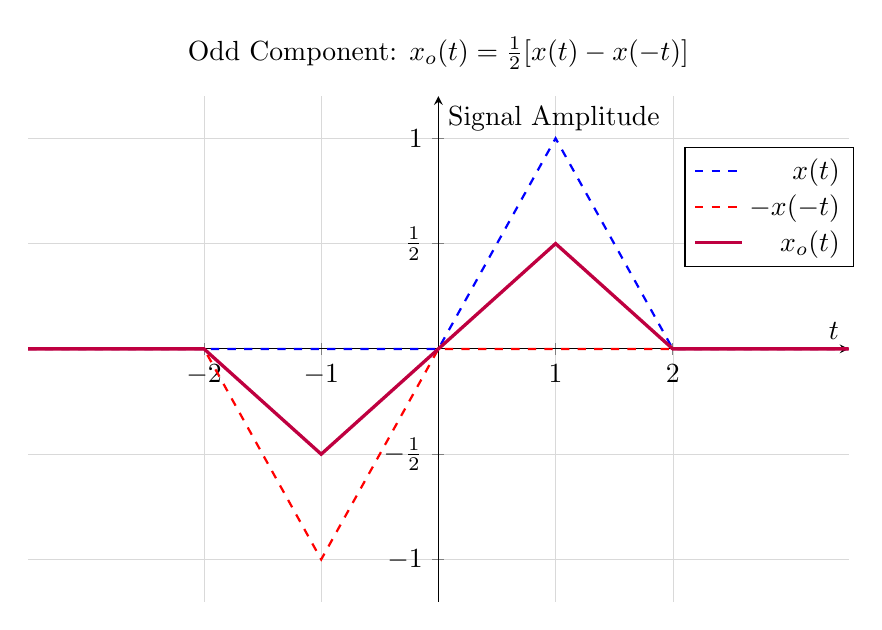
\begin{tikzpicture}
	\begin{axis}[
		% Set the overall style
		width=12cm,
		height=8cm,
		% Title with the definition of the odd component
		title={Odd Component: $x_o(t) = \frac{1}{2}[x(t) - x(-t)]$},
		% Axis labels
		xlabel={$t$},
		ylabel={Signal Amplitude},
		% Position axes at the origin
		axis lines=middle,
		% Set axis limits to show all signals
		xmin=-3.5, xmax=3.5,
		ymin=-1.2, ymax=1.2,
		% Set ticks at key points
		xtick={-2, -1, 1, 2},
		ytick={-1, -0.5, 0.5, 1},
		yticklabels={$-1$, $-\frac{1}{2}$, $\frac{1}{2}$, $1$},
		% Add a grid
		grid=major,
		grid style={line width=.1pt, draw=gray!30},
		% Position the legend
legend style={
	at={(0.8, 0.9)}, % 3% from left, 97% from bottom
	anchor=north west,   % Anchor the top-left corner of the legend
	legend cell align={right}
},
		]
		
		% 1. Plot the original signal (dashed blue)
		\addplot[blue, dashed, thick] coordinates {
			(-3.5,0) (0,0) (1,1) (2,0) (3.5,0)
		};
		\addlegendentry{$x(t)$};
		
		% 2. Plot the negative of the time-reversed signal (dashed red)
		\addplot[red, dashed, thick] coordinates {
			(-3.5,0) (-2,0) (-1,-1) (0,0) (3.5,0)
		};
		\addlegendentry{$-x(-t)$};
		
		% 3. Plot the resulting odd component (solid purple)
		\addplot[purple, very thick] coordinates {
			(-3.5,0) (-2,0) (-1,-0.5) (0,0) (1,0.5) (2,0) (3.5,0)
		};
		\addlegendentry{$x_o(t)$};
		
	\end{axis}
\end{tikzpicture}
    \caption{The odd component $x_o(t) = \frac{1}{2}[x(t)-x(-t)]$. Note its anti-symmetry about the vertical axis.}
    \label{fig:xo}
\end{figure}

\textbf{Verification:} $x_e(t) + x_o(t) = x(t)$ for all $t$.

\textbf{Answer:} $x_e(t) = \frac{1}{2}[x(t)+x(-t)]$, $x_o(t) = \frac{1}{2}[x(t)-x(-t)]$
\end{example}

\vspace{0.5em}
\hrule
\vspace{0.5em}

\begin{example}[4. Properties of a Finite-Duration Discrete-Time Signal]
\textbf{Problem:}
Consider the discrete-time signal $x[n]$ defined as:
\[
x[n] = 
\begin{cases} 
A, & n = 0, 1, 2 \\
0, & \text{otherwise}
\end{cases}
\]
where $A$ is a real constant.

Determine the following:
\begin{enumerate}
    \item The even and odd parts of $x[n]$, denoted as $x_{ev}[n]$ and $x_{od}[n]$.
    \item The total energy $E$ and average power $P_{av}$ of $x[n]$.
\end{enumerate}

\begin{figure}[H]
    \centering
    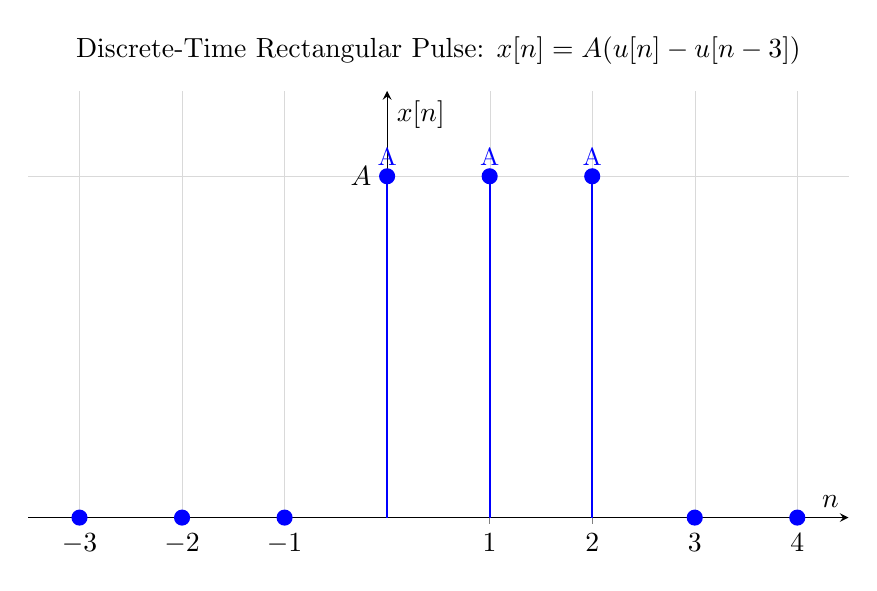
\begin{tikzpicture}
	% Define a style for our stem plots to avoid repetition
	\pgfplotsset{
		impulse/.style={
			ycomb,          % Use the 'ycomb' style for stems
			thick,          % Thickness of the stems
			mark=*,         % Marker style at the tip of the stem
			mark size=2.5pt,% Size of the marker
			blue,           % Ensure the line color is blue
			mark options={fill=blue, draw=blue}, % Explicitly set marker colors
		}
	}
	
	\begin{axis}[
		% Set the overall style
		width=12cm,
		height=7cm,
		% Title with the signal's formal definition
		title={Discrete-Time Rectangular Pulse: $x[n] = A(u[n] - u[n-3])$},
		% Axis labels
		xlabel={$n$},
		ylabel={$x[n]$},
		% Position axes at the origin
		axis lines=middle,
		% Set axis limits
		xmin=-3.5, xmax=4.5,
		ymin=0, ymax=2.5,
		% Set ticks at key points
		xtick={-3, -2, -1, 0, 1, 2, 3, 4},
		ytick={2},
		yticklabels={$A$}, % Use symbolic label 'A'
		% Add a grid
		grid=major,
		grid style={line width=.1pt, draw=gray!30},
		]
		
		% Plot the non-zero impulses and add symbolic labels above them
		\addplot[
		impulse,
		nodes near coords={A}, % Display the symbol 'A' at each point
		every node near coord/.style={anchor=south, font=\small}, % Position labels above
		] coordinates {
			(0, 2)
			(1, 2)
			(2, 2)
		};
		
		% Plot some zero-value points to show the signal's extent
		\addplot[impulse] coordinates {
			(-3, 0)
			(-2, 0)
			(-1, 0)
			(3, 0)
			(4, 0)
		};
		
	\end{axis}
\end{tikzpicture}
    \caption{The discrete-time signal $x[n]$ is non-zero only at three points, $n=0, 1, 2$, where it has a constant amplitude $A$.}
    \label{fig:signal}
\end{figure}

\textbf{Solution:}

\textbf{Part 1: Even and Odd Parts}
\[ x_{ev}[n] = \frac{1}{2}(x[n] + x[-n]), \quad x_{od}[n] = \frac{1}{2}(x[n] - x[-n]) \]

For $x[n] = A$ at $n = 0,1,2$ and $x[-n] = A$ at $n = 0,-1,-2$:

\begin{center}
\begin{tabular}{c|c|c|c|c}
$n$ & $x[n]$ & $x[-n]$ & $x_{ev}[n]$ & $x_{od}[n]$ \\
\hline
-2 & 0 & A & $A/2$ & $-A/2$ \\
-1 & 0 & A & $A/2$ & $-A/2$ \\
0 & A & A & $A$ & $0$ \\
1 & A & 0 & $A/2$ & $A/2$ \\
2 & A & 0 & $A/2$ & $A/2$ \\
\end{tabular}
\end{center}
\[ x_{ev}[n] = \begin{cases} A, & n=0 \\ A/2, & n = \pm 1, \pm 2 \\ 0, & \text{otherwise} \end{cases} \]
\[ x_{od}[n] = \begin{cases} A/2, & n = 1, 2 \\ -A/2, & n = -1, -2 \\ 0, & \text{otherwise} \end{cases} \]

\begin{figure}[H]
	\centering
	\begin{subfigure}{0.45\textwidth}
		\centering
		% Scale to a fixed height of 5cm, width is automatic
		\resizebox{!}{5cm}{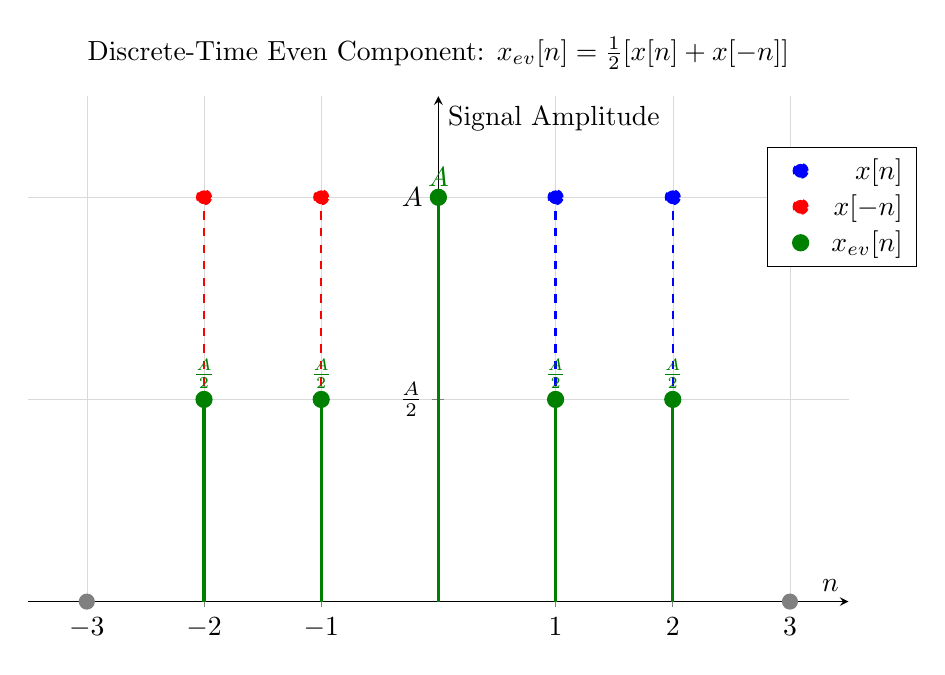
\begin{tikzpicture}
	% Define styles for the different stem plots
	\pgfplotsset{
		impulse/.style={ ycomb, thick, mark=*, mark size=2.5pt },
		original/.style={ impulse, blue, dashed },
		reversed/.style={ impulse, red, dashed },
		even/.style={ impulse, green!50!black, very thick },
	}
	
	\begin{axis}[
		% Set the overall style
		width=12cm,
		height=8cm,
		% Title with the definition of the even component
		title={Discrete-Time Even Component: $x_{ev}[n] = \frac{1}{2}[x[n] + x[-n]]$},
		% Axis labels
		xlabel={$n$},
		ylabel={Signal Amplitude},
		% Position axes at the origin
		axis lines=middle,
		% Set axis limits
		xmin=-3.5, xmax=3.5,
		ymin=0, ymax=2.5,
		% Set ticks at key points
		xtick={-3, -2, -1, 0, 1, 2, 3},
		ytick={1, 2},
		yticklabels={$\frac{A}{2}$, $A$},
		% Add a grid
		grid=major,
		grid style={line width=.1pt, draw=gray!30},
		% Position the legend
		legend style={
	at={(0.9, 0.9)}, % 3% from left, 97% from bottom
	anchor=north west,   % Anchor the top-left corner of the legend
	legend cell align={right}
},
		]
		
		% 1. Plot the original signal (dashed blue)
		\addplot[original] coordinates {(0,2) (1,2) (2,2)};
		\addlegendentry{$x[n]$};
		
		% 2. Plot the time-reversed signal (dashed red)
		\addplot[reversed] coordinates {(-2,2) (-1,2) (0,2)};
		\addlegendentry{$x[-n]$};
		
		% 3. Plot the resulting even component (solid green)
		% Plot the A/2 components with their label
		\addplot[
		even,
		nodes near coords={$\frac{A}{2}$},
		every node near coord/.style={anchor=south, font=\footnotesize},
		] coordinates {(-2,1) (-1,1) (1,1) (2,1)};
		\addlegendentry{$x_{ev}[n]$};
		
		% Plot the A component separately to give it the correct label
		\addplot[even, nodes near coords={$A$}, every node near coord/.style={anchor=south}] 
		coordinates {(0,2)};
		
		% Plot some zero-value points for context
		\addplot[impulse, gray] coordinates {(-3,0) (3,0)};
		
	\end{axis}
\end{tikzpicture}}
		\caption{Even component $x_{ev}[n]$}
	\end{subfigure}\hfill
	\begin{subfigure}{0.45\textwidth}
		\centering
		% Scale to the SAME fixed height
		\resizebox{!}{5cm}{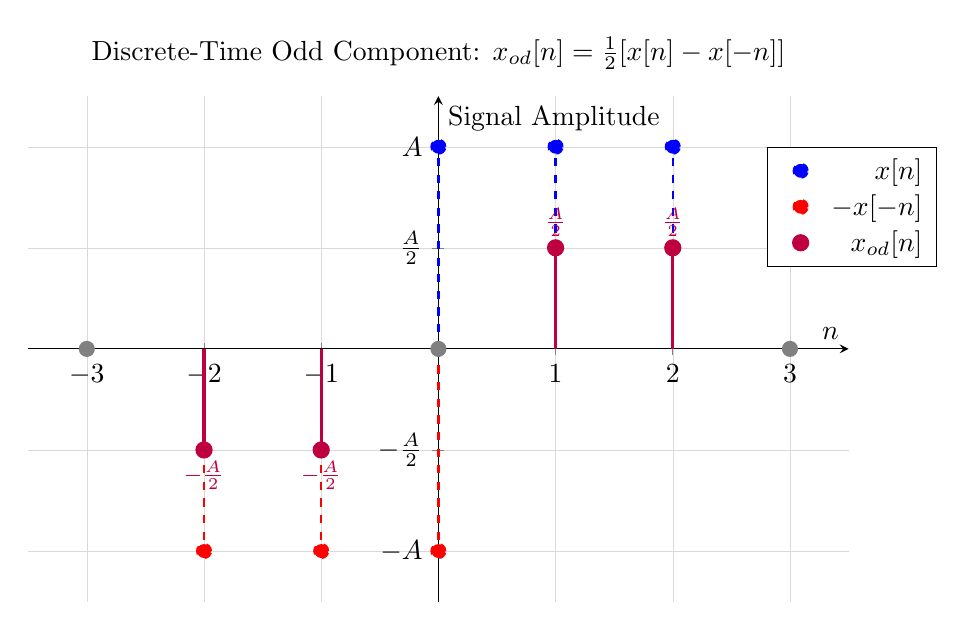
\begin{tikzpicture}
	% Define styles for the different stem plots
	\pgfplotsset{
		impulse/.style={ ycomb, thick, mark=*, mark size=2.5pt },
		original/.style={ impulse, blue, dashed },
		reversed_neg/.style={ impulse, red, dashed },
		odd/.style={ impulse, purple, very thick },
	}
	
	\begin{axis}[
		% Set the overall style
		width=12cm,
		height=8cm,
		% Title with the definition of the odd component
		title={Discrete-Time Odd Component: $x_{od}[n] = \frac{1}{2}[x[n] - x[-n]]$},
		% Axis labels
		xlabel={$n$},
		ylabel={Signal Amplitude},
		% Position axes at the origin
		axis lines=middle,
		% Set axis limits
		xmin=-3.5, xmax=3.5,
		ymin=-2.5, ymax=2.5,
		% Set ticks at key points
		xtick={-3, -2, -1, 0, 1, 2, 3},
		ytick={-2, -1, 1, 2},
		yticklabels={$-A$, $-\frac{A}{2}$, $\frac{A}{2}$, $A$},
		% Add a grid
		grid=major,
		grid style={line width=.1pt, draw=gray!30},
		% Position the legend
		legend style={
	at={(0.9, 0.9)}, % 3% from left, 97% from bottom
	anchor=north west,   % Anchor the top-left corner of the legend
	legend cell align={right}
},
		]
		
		% 1. Plot the original signal (dashed blue)
		\addplot[original] coordinates {(0,2) (1,2) (2,2)};
		\addlegendentry{$x[n]$};
		
		% 2. Plot the negative time-reversed signal (dashed red)
		\addplot[reversed_neg] coordinates {(-2,-2) (-1,-2) (0,-2)};
		\addlegendentry{$-x[-n]$};
		
		% 3. Plot the resulting odd component (solid purple)
		% Plot the positive values with labels above
		\addplot[
		odd,
		nodes near coords={$\frac{A}{2}$},
		every node near coord/.style={anchor=south, font=\footnotesize},
		] coordinates {(1,1) (2,1)};
		\addlegendentry{$x_{od}[n]$};
		
		% Plot the negative values with labels below
		\addplot[
		odd,
		nodes near coords=$-\frac{A}{2}$,
		every node near coord/.style={anchor=north, font=\footnotesize},
		] coordinates {(-2,-1) (-1,-1)};
		
		% Plot the zero-value points for context
		\addplot[impulse, gray] coordinates {(-3,0) (0,0) (3,0)};
		
	\end{axis}
\end{tikzpicture}}
		\caption{Odd component $x_{od}[n]$}
	\end{subfigure}
	\caption{Stem plots of the resulting even (left, symmetric) and odd (right, anti-symmetric) components of $x[n]$. Note that $x_{ev}[n] + x_{od}[n] = x[n]$.}
	\label{fig:evenodd}
\end{figure}

\textbf{Part 2: Energy and Power}
\[ E = \sum_{n=0}^{2} |x[n]|^2 = 3A^2 \]
\[ P_{av} = \lim_{N \to \infty} \frac{3A^2}{2N+1} = 0 \]

\textbf{Answer:} $E = 3A^2$, $P_{av} = 0$ (energy signal)
\end{example}

\vspace{0.5em}
\hrule
\vspace{0.5em}

\begin{example}[5. Properties of the Continuous-Time Unit Impulse Function]
\textbf{Problem:}
The problem consists of two parts that investigate key properties of the Dirac delta function.

\begin{enumerate}
    \item Evaluate the following integral:
    \[ x(t) = \int_{0}^{\infty} \delta(t - \sigma) \,d\sigma \]
    
    \item Show that the time-scaled unit impulse function $\delta(2t)$ is equivalent to:
    \[ \delta(2t) = \frac{1}{2}\delta(t) \]
\end{enumerate}

\textbf{Solution:}

\textbf{Part 1:} Let $\tau = t - \sigma$, then $d\tau = -d\sigma$:
\[ x(t) = \int_{0}^{\infty} \delta(t - \sigma) \,d\sigma = \int_{-\infty}^{t} \delta(\tau) \,d\tau = u(t) \]

\begin{figure}[H]
\centering
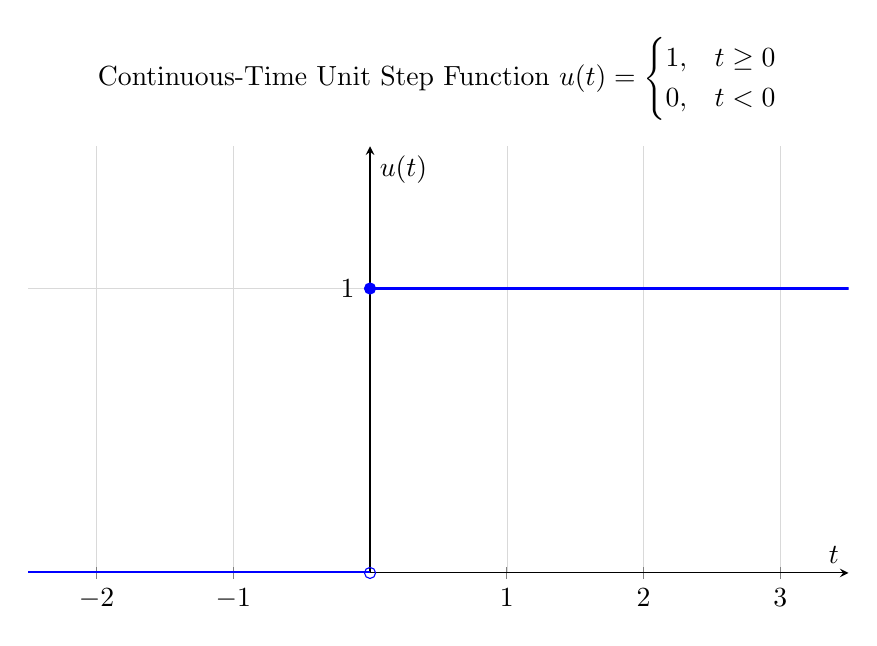
\begin{tikzpicture}
	\begin{axis}[
		% Set the overall style
		width=12cm,
		height=7cm,
		% Title with the formal piecewise definition
		title={Continuous-Time Unit Step Function $u(t) = 
			\begin{cases} 
				1, & t \ge 0 \\
				0, & t < 0
			\end{cases}$
		},
		% Axis labels
		xlabel={$t$},
		ylabel={$u(t)$},
		% Position axes at the origin
		axis lines=middle,
		% Set axis limits
		xmin=-2.5, xmax=3.5,
		ymin=0, ymax=1.5,
		% Set ticks at key points
		xtick={-2, -1, 1, 2, 3},
		ytick={1},
		% Add a grid
		grid=major,
		grid style={line width=.1pt, draw=gray!30},
		]
		
		% Draw the two parts of the function
		\draw[blue, very thick] (axis cs:-2.5, 0) -- (axis cs:0, 0);
		\draw[blue, very thick] (axis cs:0, 1) -- (axis cs:3.5, 1);
		
		% Mark the discontinuity at t=0 precisely
		% A filled circle at (0,1) indicates u(0) = 1
		\addplot[only marks, blue, mark=*, mark size=2pt] coordinates {(0,1)};
		% An open circle at (0,0) indicates the function jumps from here
		\addplot[only marks, blue, mark=o, mark size=2pt, fill=white] coordinates {(0,0)};
		
	\end{axis}
\end{tikzpicture}
\caption{The continuous-time unit step function, $u(t)$. The function is 0 for $t<0$ and 1 for $t>0$.}
\label{fig:unit_step}
\end{figure}

\textbf{Part 2:} Model $\delta(t)$ as limit of rectangular pulse $g_T(t)$ with area 1.
Time scaling: $g_T(2t)$ has width $T/2$ and height $1/T$, so area = $1/2$.
Therefore: $\delta(2t) = \frac{1}{2}\delta(t)$

\begin{figure}[H]
\centering
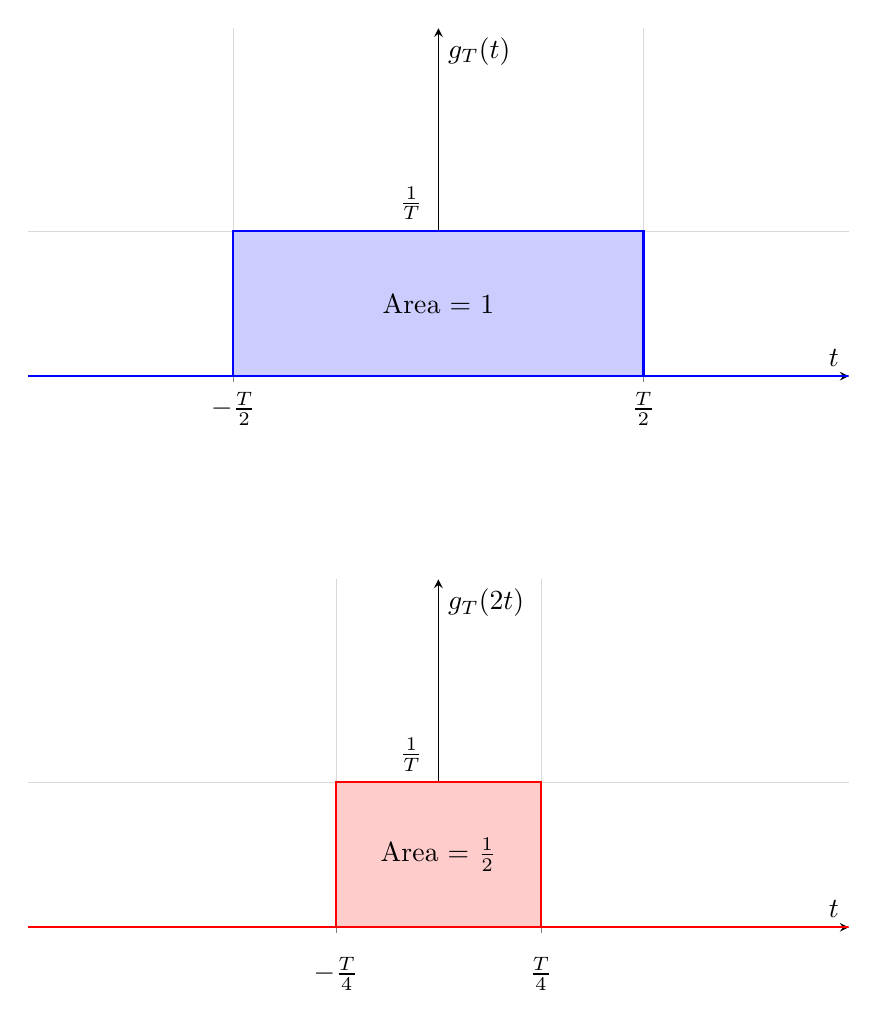
\begin{tikzpicture}
	%#################################################
	%### Top Plot: The original pulse g_T(t)
	%#################################################
	\begin{scope}[yshift=7cm]
		\begin{axis}[
			width=12cm,
			yticklabel style={yshift=10pt},
			height=6cm,
			axis lines=middle,
			xlabel={$t$},
			ylabel={$g_T(t)$},
			ymin=0, ymax=1.2,
			xmin=-2, xmax=2,
			grid=major,
			grid style={line width=.1pt, draw=gray!30},
			% removed: no marks (invalid axis key)
			xtick={-1, 1},
			xticklabels={$-\frac{T}{2}$, $\frac{T}{2}$},
			ytick={0.5},
			yticklabels={$\frac{1}{T}$},
			]
			% Plot the pulse and fill it with color
			\addplot[blue, thick, fill=blue!20, mark=none] coordinates {
				(-2,0) (-1,0) (-1,0.5) (1,0.5) (1,0) (2,0)
			} \closedcycle;
			% Add the area annotation
			\node at (axis cs:0, 0.25) {Area = $1$};
		\end{axis}
	\end{scope}
	
	%#################################################
	%### Bottom Plot: The time-scaled pulse g_T(2t)
	%#################################################
	\begin{scope}[yshift=0cm]
		\begin{axis}[
						yticklabel style={yshift=10pt},
			width=12cm,
			height=6cm,
			axis lines=middle,
			xlabel={$t$},
			ylabel={$g_T(2t)$},
			ymin=0, ymax=1.2,
			xmin=-2, xmax=2,
			grid=major,
			grid style={line width=.1pt, draw=gray!30},
			% removed: no marks (invalid axis key)
			xtick={-0.5, 0.5},
			xticklabels={$-\frac{T}{4}$, $\frac{T}{4}$},
			ytick={0.5},
			yticklabels={$\frac{1}{T}$},
			xticklabel style={yshift=-5pt},
			]
			% Plot the compressed pulse
			\addplot[red, thick, fill=red!20, mark=none] coordinates {
				(-2,0) (-0.5,0) (-0.5,0.5) (0.5,0.5) (0.5,0) (2,0)
			} \closedcycle;
			% Add the new area annotation
			\node at (axis cs:0, 0.25) {Area = $\frac{1}{2}$};
		\end{axis}
	\end{scope}
\end{tikzpicture}

\caption{Illustration of the rectangular pulse $g_T(t)$ and its time-scaled version $g_T(2t)$. The scaled pulse is half as wide, and therefore has half the area.}
\label{fig:rect_pulse}
\end{figure}

\textbf{Answer:} (1) $u(t)$, (2) $\delta(2t) = \frac{1}{2}\delta(t)$
\end{example}

\end{document}